\documentclass[11pt,a4paper]{article}
\usepackage[utf8]{inputenc}
\usepackage{amsmath}
\usepackage{amsfonts}
\usepackage{graphicx}
\usepackage[table,xcdraw]{xcolor}

\usepackage{caption}
\usepackage{subcaption}

\renewcommand{\familydefault}{\sfdefault} % cambiamos la fuente a una sans

\usepackage{float} % para que floten las imagenes o algo asi...
\usepackage{wallpaper} %paquete para usar una imagen como encabezado!
\usepackage{hyperref} %para usar hypervinculos 
\usepackage[export]{adjustbox} %para usar marcos en imagenes
\usepackage{eurosym} % para el euro
\usepackage{transparent} %para las marcas de agua
\usepackage{eso-pic}  %para las marcas de agua

\definecolor{azul_marcos}{RGB}{0,128,159} %defino el color azul de los marcos
\usepackage{sectsty} %esto es para cambiar el color de las fuentes creo
\renewcommand{\familydefault}{\sfdefault} % cambiamos la fuente a una sans
\sectionfont{\color{azul_marcos}}  % sets colour of sections
\subsectionfont{\color{azul_marcos}}  % sets colour of sections


\usepackage{pdfpages} %para insertar pdfs
\usepackage{amssymb}
\usepackage{pstcol} % para color
\usepackage{pst-node} % para diagramas
\usepackage{pst-plot} % para representacion de dat
\usepackage[spanish]{babel}
\addto\captionsspanish{\renewcommand\chaptername{Bloque}}
%\usepackage[total={18cm,21cm},top=2cm, left=2cm]{geometry}
\usepackage{anysize}
\pagestyle{plain}
%\markboth{left head}{right head}
%\markright{Guía de impresión ABS Tech}
\marginsize{3cm}{2cm}{2.5cm}{1cm}
\title{Guía de impresión ABS Tech}
\date{}

%configuracion de la marca de agua
\AddToShipoutPicture{
    \put(0,0){
        \parbox[b][\paperheight]{\paperwidth}{%
            \vfill
            \centering
            {\transparent{0.1}
\includegraphics[scale=1.25]{FOTOS/logofff}}%
            \vfill
        }
    }
}

\begin{document}
\ULCornerWallPaper{1}{FOTOS/header}
\LLCornerWallPaper{1}{FOTOS/footer}
%\maketitle
%\tableofcontents

\includepdf{PDF/PORTADA.pdf}
\section{¿Qué es ABS Tech?}ABS Tech es un filamento para impresión 3D FFF/FDM de acrilonitrilo butadieno estireno (A.B.S.) especialmente tratado con aditivos para reducir el efecto warping característico de éste material y hacerlo más fácil de usar.
\section{¿Por qué usar ABS Tech?}
ABS Tech amplía las posibilidades de los filamentos de ABS tradicionales manteniendo a la vez las propiedades químicas y mecánicas de este fantástico termoplástico.
\begin{itemize}
\item Su tratamiento anti-warping permite la impresión de volúmenes más grandes que los habituales y un mejor aprovechamiento en impresoras domésticas.
\item Los olores producidos por nuestro ABS Tech son menos molestos que los de otros filamentos de ABS.
\item ABS Tech es un material muy tenaz, duro y con buena resistencia química a la abrasión.
\item Es soluble en acetona. Esto permite unir piezas de ABS fuertemente usando acetona como pegamento.
\item Por último las piezas impresas en ABS Tech se pueden postprocesar con facilidad ya que éste material puede ser taladrado, lijado, pintado, etc...
\end{itemize}
\section{Ficha técnica y parámetros de impresión}
\begin{table}[H]
\centering
\caption*{Ficha técnica}
\begin{tabular}{|
>{\columncolor[HTML]{FFFFFF}}l |
>{\columncolor[HTML]{FFFFFF}}c |}
\hline
\multicolumn{1}{|c|}{\cellcolor[HTML]{FFFFFF}\textbf{Material}}   & Acrilonitrilo Butadieno Estireno   \\ \hline
\textbf{Colores disponibles}              & 22                 \\ \hline
\textbf{Formatos disponibles}             & 1kg, 250gr         \\ \hline
\textbf{Temperatura de deflexión térmica} & 88ºC               \\ \hline
\textbf{Temperatura de fusión}            & 200ºC              \\ \hline
\textbf{Temperatura de descomposición}    & \textgreater 260ºC \\ \hline
\textbf{Densidad}                         & 1.05 gr / cm3      \\ \hline
\textbf{Resistencia al impacto}                         & 17 kg-cm / cm3      \\ \hline
\textbf{Estiramiento máximo}              & 25\%              \\ \hline
\end{tabular}
\end{table}
\begin{table}[H]
\centering
\begin{tabular}{|
>{\columncolor[HTML]{FFFFFF}}l |
>{\columncolor[HTML]{FFFFFF}}c |}
\hline
\multicolumn{1}{|c|}{\cellcolor[HTML]{FFFFFF}\textbf{Temperatura recomendada de impresión}} & 240º-245º              \\ \hline
\textbf{Velocidad recomendada de impresión}                         & 50-90mm/s              \\ \hline
\textbf{Temperatura cama caliente}                                  &  80º - 100º        \\ \hline
\textbf{Ventilador de capa}                                      & Desactivado o a baja velocidad                 \\ \hline
\textbf{Velocidad de la primera capa}                                                 & 20 mm/s                      \\ \hline
\textbf{Altura de la primera capa}                                           & \textgreater 0.2 mm                      \\ \hline
\end{tabular}
\end{table}

Puedes descargarte nuestros perfiles completos de impresión de los principales programas de laminación (Cura, Slic3r y Simplify3D) desde nuestra página web:
\\\\
\centerline{ {\huge \url{www.fffworld.com/documentation} } }
\\\\
Los parámetros óptimos dependerán de la impresora 3D que utilices, sin embargo, son unos buenos parámetros para tenerlos como punto de partida. Con unas pocas impresiones serás capaz de encontrar los límites y la configuración perfecta para tu maquina.
\section{Problemas y soluciones}
	\subsection{El warping y el cracking}
		\subsubsection{¿Qué son?}El ABS es un material ideal para imprimir en 3D por su disponibilidad y características: se extruye a una temperatura ligeramente superior al PLA, es menos exigente con el tipo de hot-end utilizado, es menos propenso a atascos puesto que no se cristaliza al degradarse y posee propiedades mecánicas superiores.
\\\\
Su mayor desventaja es el conocido efecto warping/craking, sin embargo con los consejos adecuados estos problemas pueden superarse.
\\\\
El efecto warping es el nombre que recibe en el mundo de la impresión 3D la problemática causada por la contracción del plástico al enfriarse que en ocasiones provoca que las piezas se deformen o se rompan.
\\\\
Se distingue entre warping y cracking según el problema afecte a la primera capa o a capas intermedias de la pieza.
%EJEMPLO_WARPING
%Leyenda: Ejemplo de problema de warping
%EJEMPLO_CRACKING
%Leyenda: Ejemplo de problema de cracking
\begin{figure}[H]
    \centering
    \begin{subfigure}[b]{0.4\textwidth}
        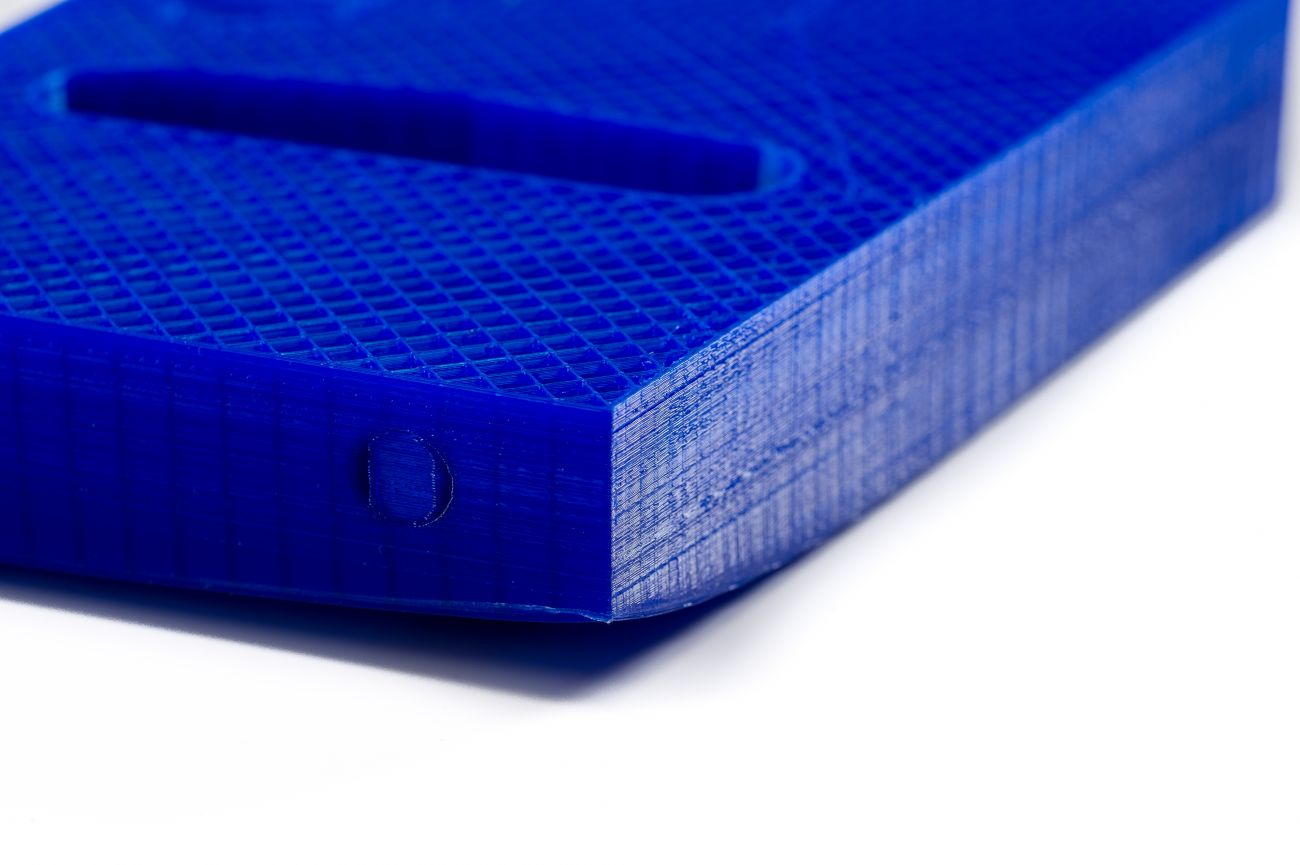
\includegraphics[width=\textwidth,cfbox=azul_marcos 4pt 0pt]{FOTOS/EJEMPLO_WARPING}
	\caption*{Ejemplo de problema de warping}
    \end{subfigure}
    \qquad %add desired spacing between images, e. g. ~, \quad, \qquad, \hfill etc. 
      %(or a blank line to force the subfigure onto a new line)
    \begin{subfigure}[b]{0.4\textwidth}
        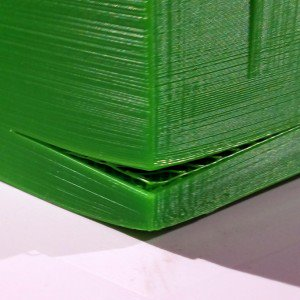
\includegraphics[width=\textwidth,cfbox=azul_marcos 4pt 0pt]{FOTOS/EJEMPLO_CRACKING}
	\caption*{Ejemplo de problema de cracking}
    \end{subfigure}   
\end{figure}
		\subsubsection{¿Cuáles son sus causas?}Imprimir en 3D supone depositar hilos de filamento que se pegan entre sí y construyen las piezas deseadas.
\\\\
Al enfriarse estos hilos se contraen reduciendo su longitud y provocan tensiones acumulativas en las piezas con efectos indeseados.
\\\\
Las distintas fases del problema pueden observarse en la imagen:
%CAUSA WARPING
\begin{figure}[H]
\centering
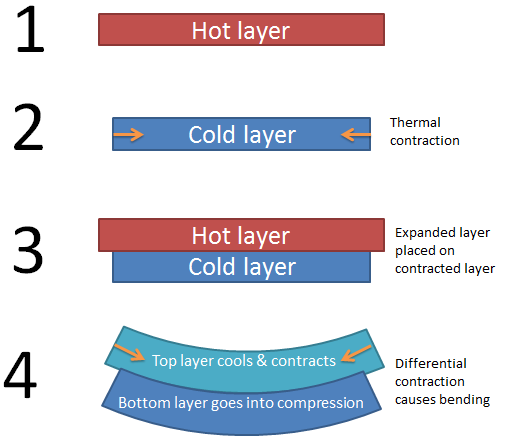
\includegraphics[width=0.6\textwidth,cfbox=azul_marcos 4pt 0pt]{FOTOS/CAUSA_WARPING_1}
\end{figure}

\begin{description}
\item[1] La primera capa se deposita caliente: Al estar todavía caliente su tamaño es superior al que tendrá a temperatura ambiente.
\item[2] La primera capa se enfría: Al enfriarse se contrae reduciendo su tamaño y aparecen las primeras tensiones que tienden a despegar la pieza de la superficie de impresión.
\item[3] La segunda capa se deposita caliente: Al estar caliente, el volumen de la segunda capa es mayor que el de la primera.
\item[4] La segunda capa se enfría: La tensión generada por la contracción de la segunda capa se suma a la provocada por la primera capa y la pieza se despega curvándose.
\end{description}
			\paragraph{La influencia de la temperatura en el warping}\mbox{}\\\\
La diferencia de temperatura es por tanto la responsable del problema, en concreto la diferencia entre la temperatura ambiente y la temperatura de transición vítrea del material.
\\\\
\url{https://en.wikipedia.org/wiki/Glass_transition}
\\\\
La temperatura de transición vítrea del ABS es de unos 100º y la temperatura ambiente suele estar entorno a los 30º, es ese salto de 70º el que produce el problema.
\\\\
Como curiosidad merece la pena explicar que el PLA se dilata más que el ABS con la temperatura sin embargo su transición vítrea se sitúa en los 60º y, como la diferencia con la temperatura ambiente es mucho menor, no se ve afectado por el warping.
\\\\
Por lo tanto controlando la temperatura ambiente podemos controlar totalmente el warping, aunque esto no siempre es sencillo.
		\subsubsection{Soluciones físicas}
			\paragraph{Mejorar la adherencia de la superficie de impresión}\mbox{}\\\\
El efecto warping se puede atenuar mejorando la adherencia de la superficie de impresión, sin embargo esta no es la mejor solución puesto que no ataca a la raíz del problema y no haríamos nada para solucionar el cracking.
\\\\
%CAUSA WARPING 2
\begin{figure}[H]
\centering
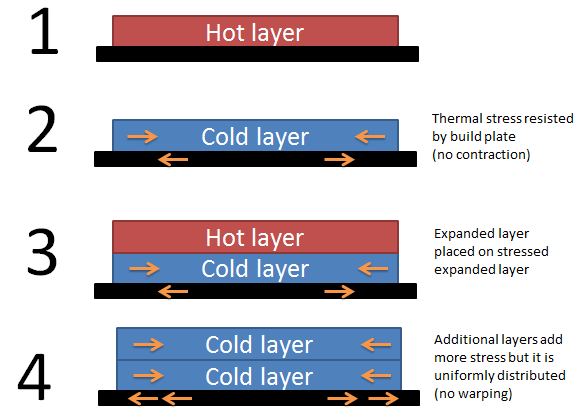
\includegraphics[width=0.6\textwidth,cfbox=azul_marcos 4pt 0pt]{FOTOS/CAUSA_WARPING_2}
\end{figure}

\begin{description}
\item[1] La primera capa se deposita caliente: Al estar todavía caliente su tamaño es superior al que tendrá a temperatura ambiente.
\item[2] La primera capa se enfría: Al enfriarse la primera capa tienda a contraerse, sin embargo la adherencia de la superficie contraresta ésta fuerza.
\end{description}
Aplicando un producto adhesivo no se eliminarán las tensiones producidas por el enfriamiento del ABS, pero pueden contrarrestarse y es una solución eficaz para piezas pequeñas.
\\\\
Es muy importante que la superficie esté libre de polvo, grasa u elementos extraños que afecten negativamente a la adherencia.
\\\\
También es necesario que la superficie de impresión esté perfectamente nivelada para que la primera capa tenga una altura uniforme.
\\\\
Entre los productos más usados y con mejores resultados podemos encontrar:

				\subparagraph{Cinta kapton}\mbox{}\\\\
Se trata de una cinta adhesiva de poliamida con pegamento de silicona preparada para soportar altas temperaturas. El ABS se pega bastante bien a este tipo de cinta y se ha usado ampliamente en impresión 3D con este propósito. Para utilizarla correctamente hay que pegarla con cuidado a la superfie de impresión.
%KAPTON1 KAPTON2
\begin{figure}[H]
    \centering
    \begin{subfigure}[b]{0.4\textwidth}
        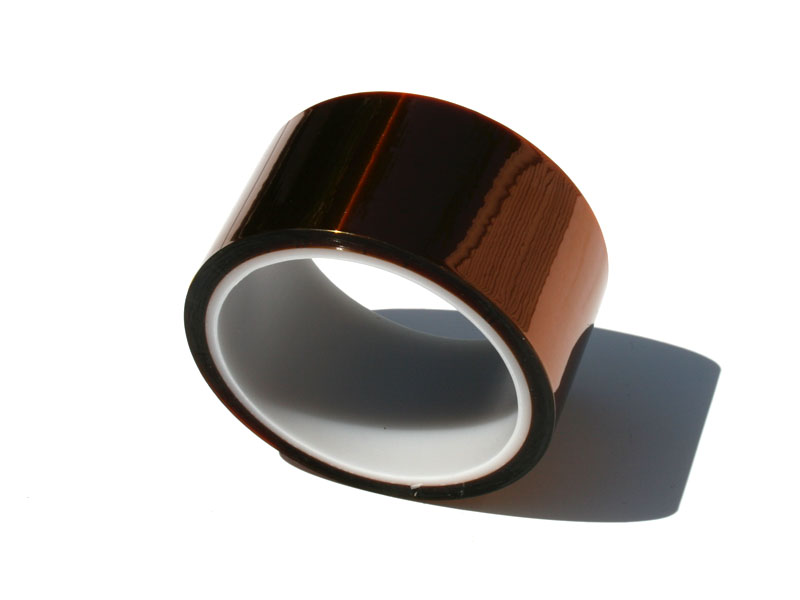
\includegraphics[width=\textwidth,cfbox=azul_marcos 4pt 0pt]{FOTOS/KAPTON1}
	\caption*{Rollo de cinta Kapton}
    \end{subfigure}
    \qquad %add desired spacing between images, e. g. ~, \quad, \qquad, \hfill etc. 
      %(or a blank line to force the subfigure onto a new line)
    \begin{subfigure}[b]{0.4\textwidth}
        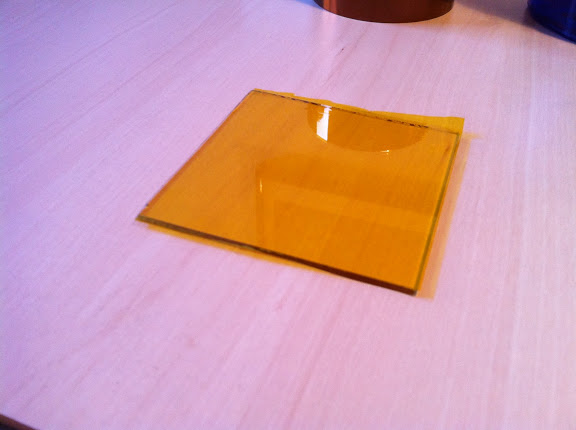
\includegraphics[width=\textwidth,cfbox=azul_marcos 4pt 0pt]{FOTOS/KAPTON2}
	\caption*{Cristal con Kapton}
    \end{subfigure}   
\end{figure}
				\subparagraph{Laca}\mbox{}\\\\
La laca ha demostrado ser un recurso eficaz a la hora de incrementar la adherencia de la superficie de impresión. Es recomendable elegir una laca que contenga los menos aditivos posibles. La forma de utilizarla es pulverizar abundante sobre la superficie de impresión antes de imprimir.
%LACA
\begin{figure}[H]
\centering
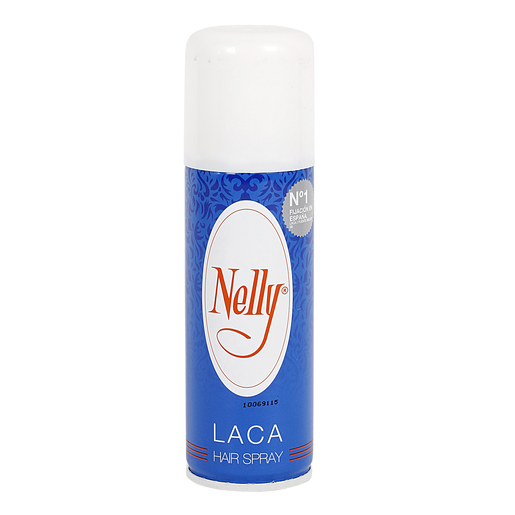
\includegraphics[width=0.3\textwidth,cfbox=azul_marcos 4pt 0pt]{FOTOS/LACA}
\caption*{Laca Nelly}
\end{figure}
				\subparagraph{Disolución ABS-Acetona}\footnote{ADVERTENCIA: Este método puede ser tan eficaz que la pieza resultante no pueda ser despegada de la base sin romper alguna de las dos} \mbox{}\\\\
Aprovechando la solubilidad del ABS en acetona puede prepararse una solución para pegar fuertemente las piezas a la superficie de impresión. Se trata sumergir pedazos de ABS en acetona y dejar que ésta disuelva el plástico. Una vez disuelto, el líquido resultante puede aplicarse con un pincel sobre la superficie de impresión para aumentar notáblemente la adherencia.
				\subparagraph{Otros productos}\mbox{}\\\\
Además de los métodos mencionados hay usuarios que utilizan otros para conseguir los mismos objetivos. Por otra parte, el avance de la impresión 3D ha propiciado la aparición de productos específicos para solucionar los problemas de adherencia. Consideramos que los métodos anteriormente expuestos son los más asequibles y eficaces, sin embargo queremos mencionar algunos otros por si pueden serte de ayuda:
\begin{description}
\item[Superficies de impresion] 3M BlueTape, Buildtak
\item[Productos adhesivos] Fixwarp3d, 3DLAC, Dimafix, Pegamento de barra UHU (PVA)
\end{description}
			\paragraph{Utilización de cama caliente}\mbox{}\\\\
Utilizar una superficie de impresión calefactada (cama caliente) es necesario para imprimir ABS de forma satisfactoria y son muchas las impresoras que incorporan una.
\begin{figure}[H]
\centering
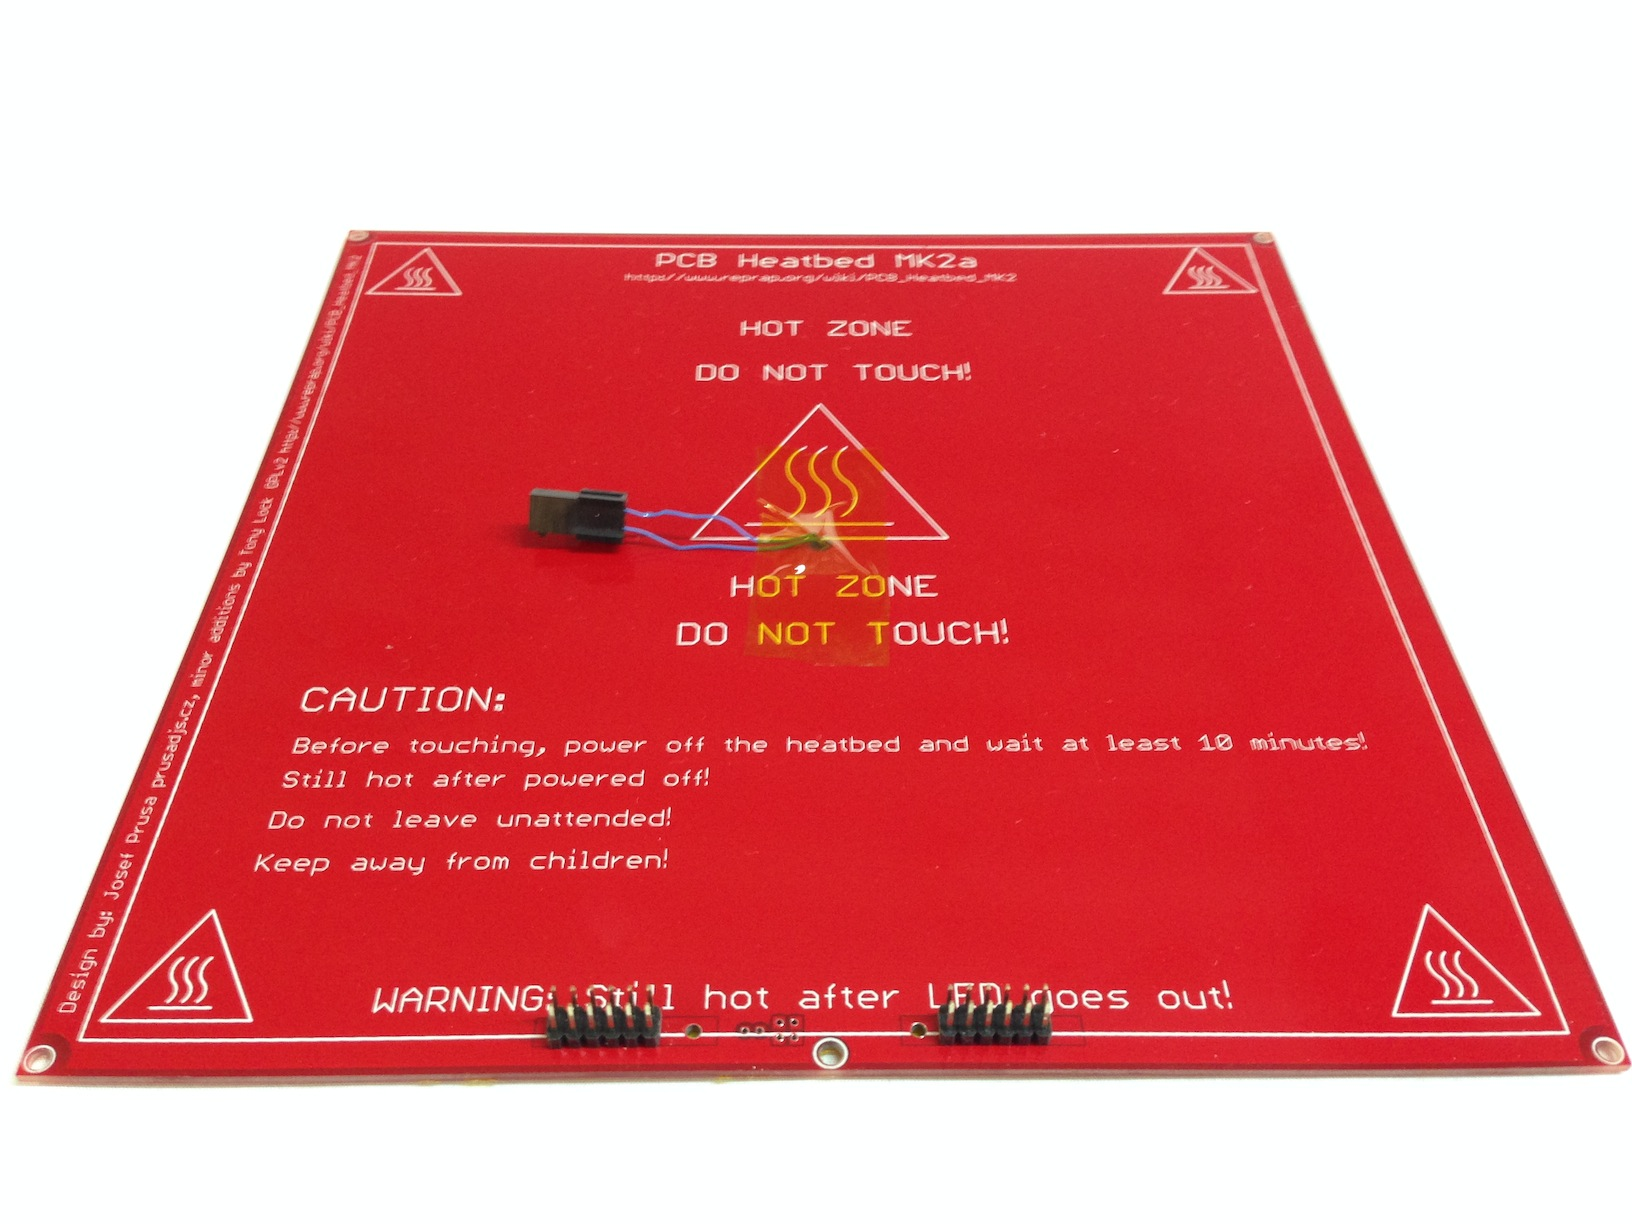
\includegraphics[width=0.6\textwidth,cfbox=azul_marcos 4pt 0pt]{FOTOS/HEATEDBED}
\caption*{Cama caliente para impresora RepRap}
\end{figure}
La cama caliente va a asegurar que las primeras capas se mantengan a una temperatura suficiente para evitar la contracción del material y los problemas de warping.
\\\\
La cama caliente debe calentarse al menos a 80º aunque es recomendable que esté al menos a 100º.
\\\\
Hay que tener en cuenta que la cama caliente no alcanza a mantener la temperatura de las capas superiores en piezas grandes por tanto aún puede producirse cracking en volúmenes grandes.
			\paragraph{Evitar corrientes de aire}\mbox{}\\\\
Para evitar que la pieza pueda enfriarse bruscamente es muy conveniente imprimir en áreas aisladas de corrientes de aire. Esto entra en conflicto con la recomendación de imprimir en areas ventiladas para evitar la acumulación de gases nocivos.
\\\\
Por tanto la mejor opción pasa por encerrar la impresora en un recinto que permita mantener la temperatura y evitar corrientes de aire.
% CERRAMIENTO1  CERRAMIENTO2  CERRAMIENTO3 
\begin{figure}[H]
    \centering
    \begin{subfigure}[b]{0.3\textwidth}
        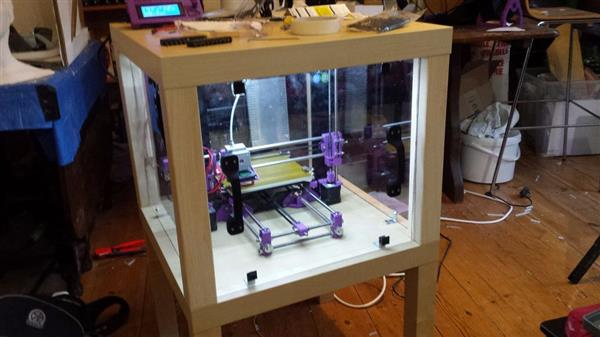
\includegraphics[width=\textwidth,cfbox=azul_marcos 4pt 0pt]{FOTOS/CERRAMIENTO1}
    \end{subfigure}
    \quad %add desired spacing between images, e. g. ~, \quad, \qquad, \hfill etc. 
      %(or a blank line to force the subfigure onto a new line)
    \begin{subfigure}[b]{0.3\textwidth}
        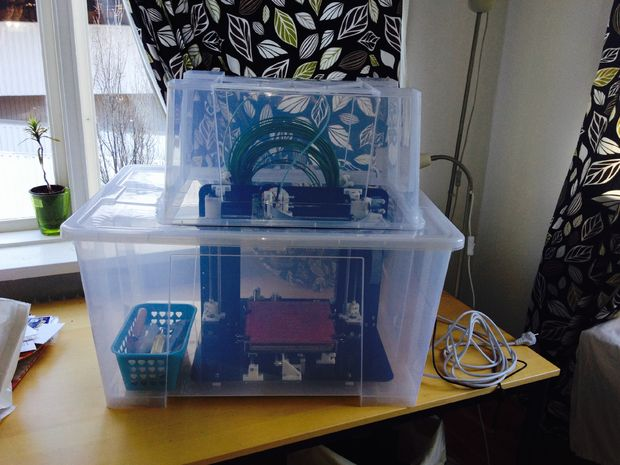
\includegraphics[width=\textwidth,cfbox=azul_marcos 4pt 0pt]{FOTOS/CERRAMIENTO2}
    \end{subfigure}
    \quad %add desired spacing between images, e. g. ~, \quad, \qquad, \hfill etc. 
    %(or a blank line to force the subfigure onto a new line)
    \begin{subfigure}[b]{0.3\textwidth}
        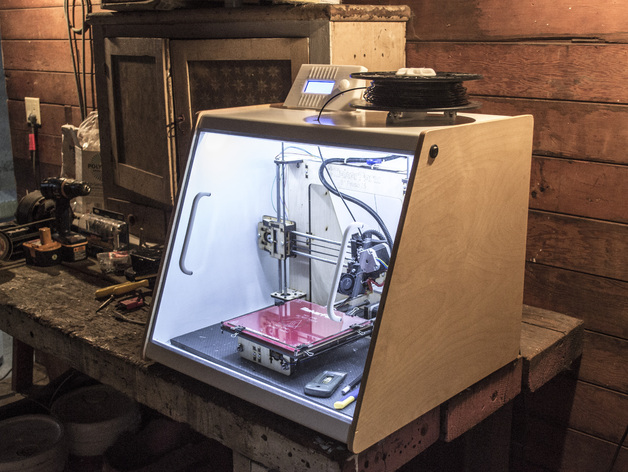
\includegraphics[width=\textwidth,cfbox=azul_marcos 4pt 0pt]{FOTOS/CERRAMIENTO3}
    \end{subfigure}
    \caption*{Ejemplos de cerramientos caseros}
\end{figure}
Por su parte son muchas las impresoras que están diseñadas en forma de caja y no necesitan de este aislamiento adicional.
% IMPRESORACERRADA1	IMPRESORACERRADA2	IMPRESORACERRADA3
\begin{figure}[H]
    \centering
    \begin{subfigure}[b]{0.3\textwidth}
        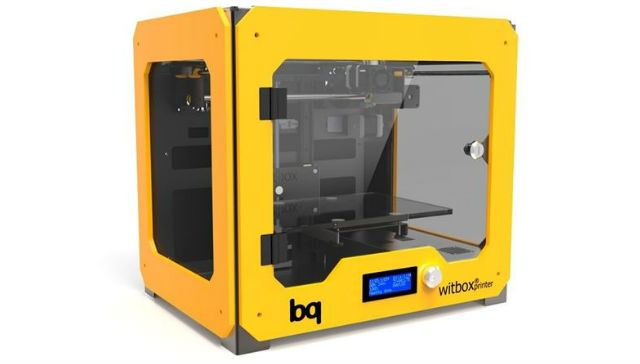
\includegraphics[width=\textwidth,cfbox=azul_marcos 4pt 0pt]{FOTOS/IMPRESORACERRADA1}
    \end{subfigure}
    \quad %add desired spacing between images, e. g. ~, \quad, \qquad, \hfill etc. 
      %(or a blank line to force the subfigure onto a new line)
    \begin{subfigure}[b]{0.3\textwidth}
        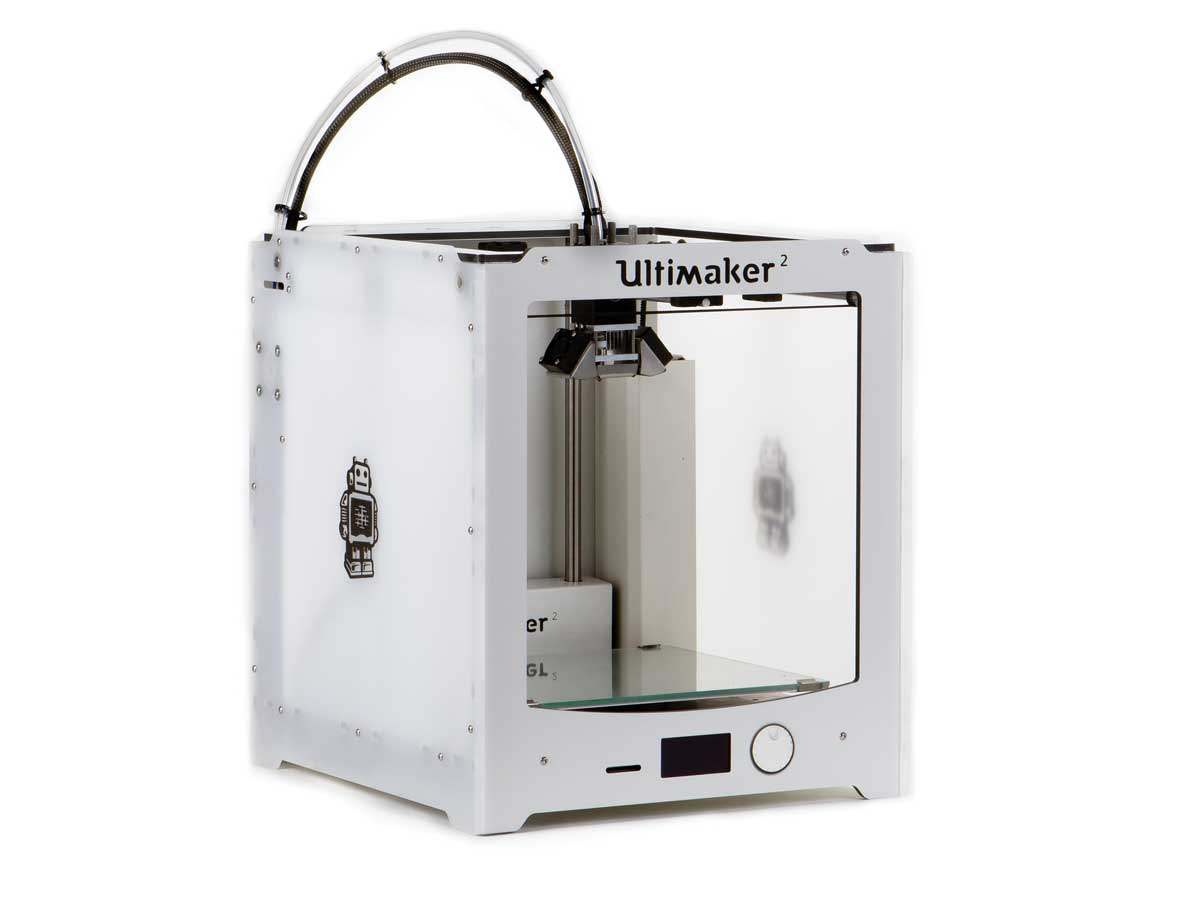
\includegraphics[width=\textwidth,cfbox=azul_marcos 4pt 0pt]{FOTOS/IMPRESORACERRADA2}
    \end{subfigure}
    \quad %add desired spacing between images, e. g. ~, \quad, \qquad, \hfill etc. 
    %(or a blank line to force the subfigure onto a new line)
    \begin{subfigure}[b]{0.3\textwidth}
        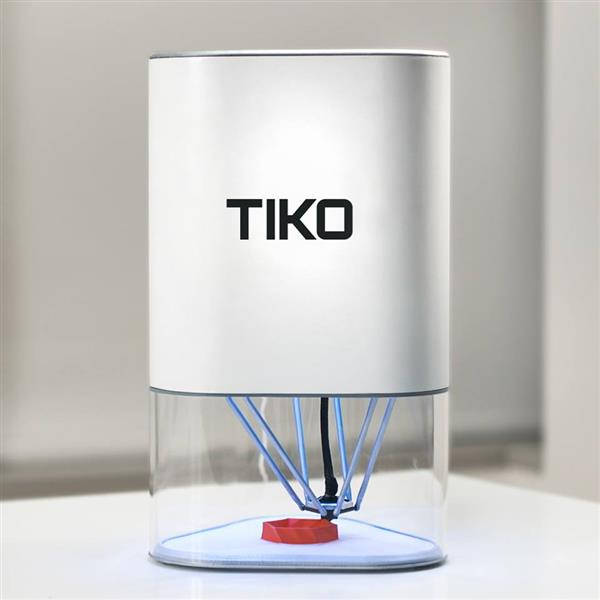
\includegraphics[width=\textwidth,cfbox=azul_marcos 4pt 0pt]{FOTOS/IMPRESORACERRADA3}
    \end{subfigure}
    \caption*{Ejemplos de impresoras cerradas}
\end{figure}
			\paragraph{Calefactar el recinto}\mbox{}\\\\
Las impresoras industriales y profesionales imprimen ABS en un recinto calefactado que mantiene la pieza a 80º durante toda la impresión. Esto requiere de ingeniería extra para refrigerar el hot-end y el resto de componentes, pero elimina por completo los problemas de warping y cracking.
\\\\
% STRATASYS
\begin{figure}[H]
\centering
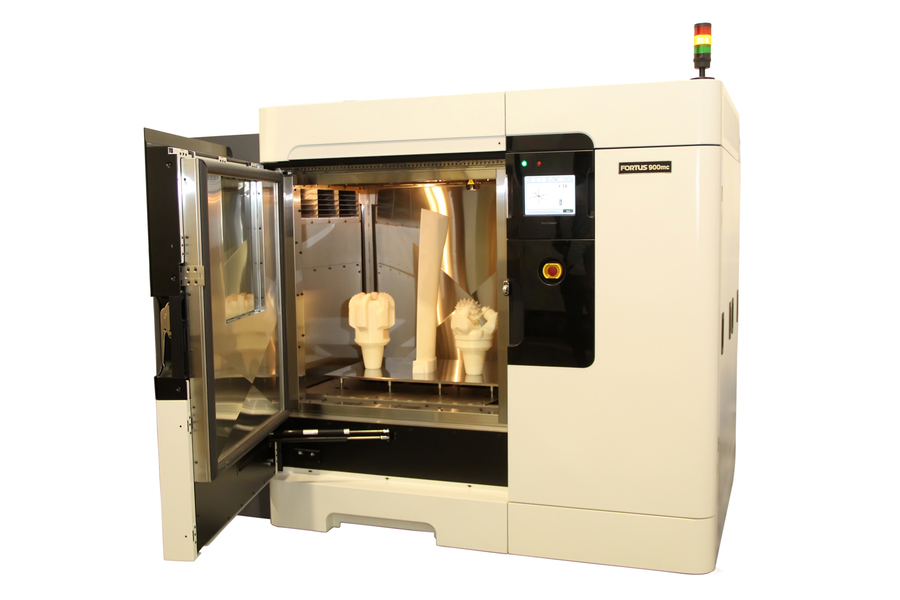
\includegraphics[width=0.6\textwidth,cfbox=azul_marcos 4pt 0pt]{FOTOS/STRATASYS}
\caption*{Impresora industrial con recinto calefactado}
\end{figure}
Aunque este tipo de impresoras no están al alcance del usuario doméstico las mencionamos para una mejor comprensión del problema.
		\subsubsection{Soluciones de software y de diseño}Además de todo lo comentado anteriormente existen técnicas de diseño y laminado que permiten reducir o eliminar los problemas de warping.
			\paragraph{Brim y raft}\mbox{}\\\\
El brim y el raft son opciones que ofrecen los programas de laminado para aumentar la adherencia de las piezas a la base.
%BRIM			RAFT 	
% Leyenda: Brim	Leyenda: Raft
\begin{figure}[H]
    \centering
    \begin{subfigure}[b]{0.4\textwidth}
        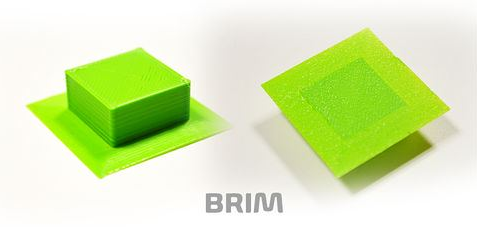
\includegraphics[width=\textwidth,cfbox=azul_marcos 4pt 0pt]{FOTOS/BRIM}
    \end{subfigure}
    \qquad %add desired spacing between images, e. g. ~, \quad, \qquad, \hfill etc. 
      %(or a blank line to force the subfigure onto a new line)
    \begin{subfigure}[b]{0.4\textwidth}
        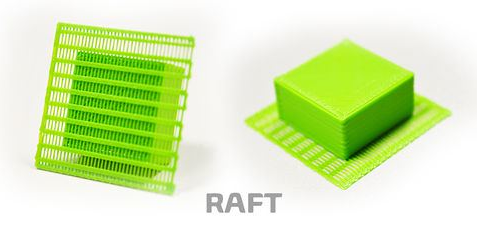
\includegraphics[width=\textwidth,cfbox=azul_marcos 4pt 0pt]{FOTOS/RAFT}
    \end{subfigure}   
\end{figure}
La opción Brim crea unos perímetros extras alrededor de la pieza para aumentar la superficie y mejorar la adhesión.
\\\\
Por su parte la opción Raft crea una especie de cama de varias capas de grosor para después imprimir la pieza sobre dicha cama.
\\\\
En general es preferible la utilización de Brim ya que es más rápido.
\\\\
Para más información acerca de cómo activar y usar estas opciones en su programa de laminado puedes consultar los siguientes enlaces:\\\\
\url{http://manual.slic3r.org/expert-mode/skirt}\\\\
\url{https://www.simplify3d.com/support/tutorials/rafts-skirts-and-brims/}\\\\
\url{https://ultimaker.com/en/resources/16525-platform-adhesion}
			\paragraph{Impacto del infill en el warping}\mbox{}\\\\
El grado de warping es directamente proporcional a la cantidad de plástico contrayéndose, por esto porcentajes de infill más bajos producen menos warping que piezas con más relleno.
\\\\
El tamaño de las primeras capas afecta de la misma manera que el infill y puede ser recomendable reducir el grosor o el número las mismas.
			\paragraph{Modificación de piezas para reducir el warping}
				\subparagraph{Añadir soportes en las esquinas}\mbox{}\\\\
Un método de controlar el warping es rediseñar la pieza reforzando los puntos por dónde se ha despegado de cama.
\\\\
Si tras una impresión fallida comprobamos que una o varias esquinas siguen levantándose sin remedio puede ser necesario añadir un soporte en dicha zona.
\\\\
El soporte deberá ser más o menos grande dependiendo de la gravedad del problema.
%	MOUSEEAR1			MOUSEEAR2
\begin{figure}[H]
    \centering
    \begin{subfigure}[b]{0.4\textwidth}
        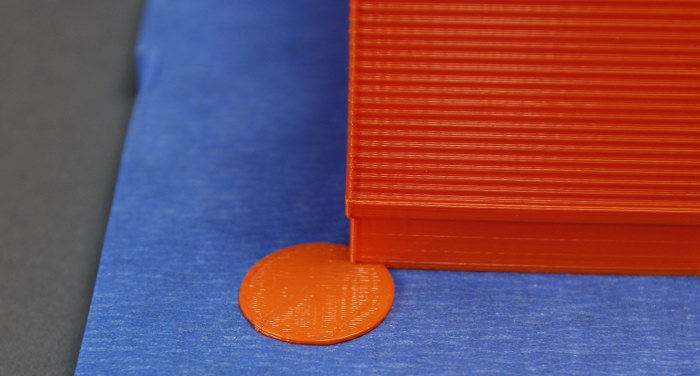
\includegraphics[width=\textwidth,cfbox=azul_marcos 4pt 0pt]{FOTOS/MOUSEEAR1}
    \end{subfigure}
    \qquad %add desired spacing between images, e. g. ~, \quad, \qquad, \hfill etc. 
      %(or a blank line to force the subfigure onto a new line)
    \begin{subfigure}[b]{0.4\textwidth}
        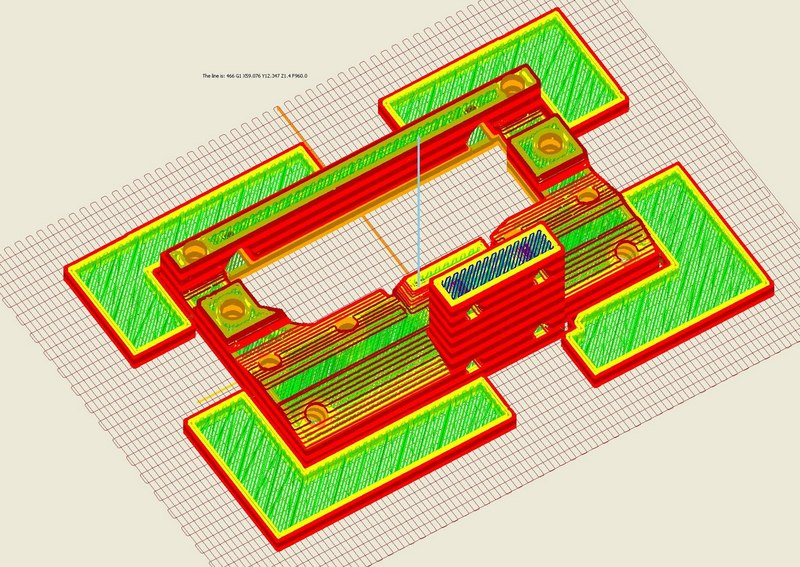
\includegraphics[width=\textwidth,cfbox=azul_marcos 4pt 0pt]{FOTOS/MOUSEEAR2}
    \end{subfigure}   
\end{figure}	
				\subparagraph{Evitar esquinas redondeadas}\mbox{}\\\\
Se ha comprobado que el warping afecta más a las esquinas redondas y a las piezas con base circular o perímetros convexos.
\\\\
Si estás teniendo este problema tu pieza puede beneficiarse de un rediseño que elimine dichas geometrías problemáticas.
			\paragraph{Bajar la velocidad y la altura de la primera capa}\mbox{}\\\\
Es muy importante que la primera capa quede lo mejor adherida posible a la superficie de impresión.
\\\\
Para conseguirlo es recomendable reducir notablemente la velocidad de la primera capa favoreciendo que el material se pegue de manera más firme y uniforme a la base.
\\\\
Una velocidad de 20 mm/s en la primera capa debería ser suficiente para alcanzar dicho objetivo. También es recomendable reducir la altura de la primera capa de forma que no supere los 0.2 mm.
			\paragraph{Uso de ventilador de capa}\mbox{}\\\\
El ventilador de capa se encarga de enfriar el plástico tras su extrusión y esto es precisamente lo que hay que evitar al imprimir ABS.
\\\\
Por ello como norma general se recomienda desactivarlo para imprimir ABS.
\\\\
No obstante puede usarse de forma selectiva en algunos momentos de la impresión si tu software de laminado lo permite.
\\\\
En todo caso si vas a utilizarlo te recomendamos que lo hagas a una velocidad inferior a la  habitual.
	\subsection{Los vapores tóxicos}Se sabe que el ABS emite vapores nocivos al ser impreso que pueden ser potencialmente dañinos para los humanos.
\\\\
Por eso se recomienda que la impresora esté en un lugar ventilado o al menos no permanecer junto a ella de manera prolongada durante el proceso de impresión.
\\\\
Si vas a utilizar ABS de forma intensiva puede ser interesante instalar un sistema de filtrado y extracción en su impresora para evitar completamente la exposición a estos vapores.
% VENTILACIONVAPORES
\begin{figure}[H]
\centering
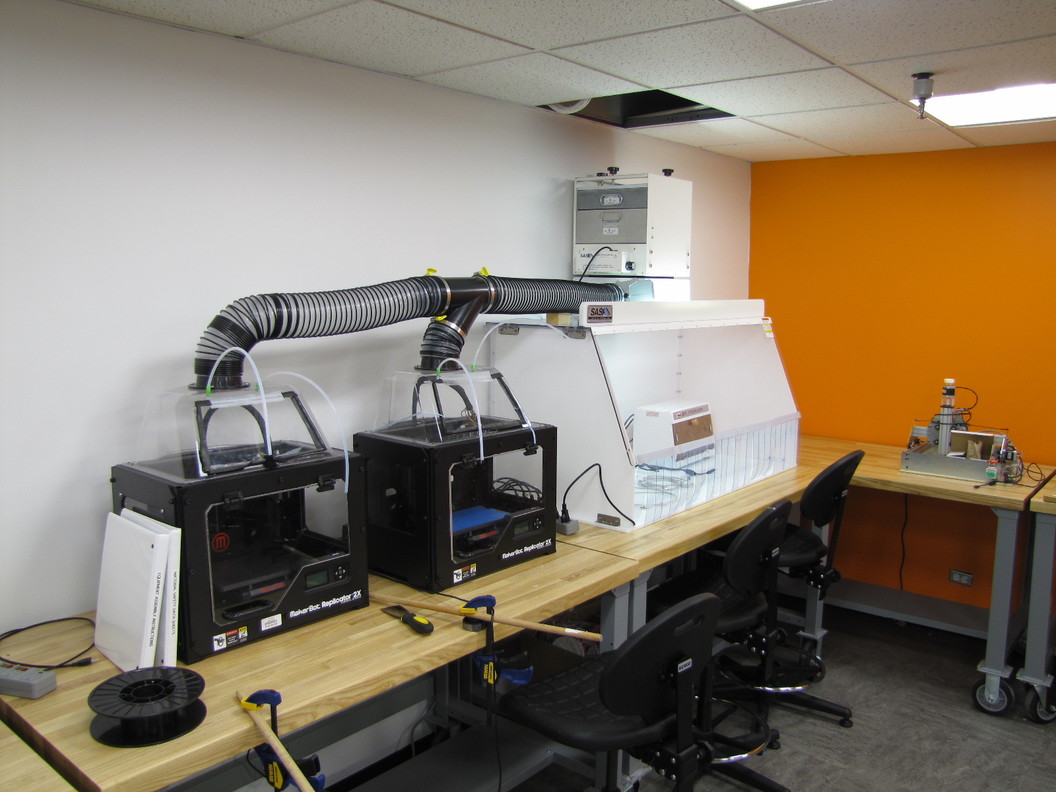
\includegraphics[width=0.5\textwidth,cfbox=azul_marcos 4pt 0pt]{FOTOS/VENTILACIONVAPORES}
\caption*{Sistema de filtrado y extracción}
\end{figure}
\section{Consejos de impresión: El postprocesado del ABS}
	\subsection{Lijar, cortar y taladrar}Una de las ventajas del ABS es su facilidad de postprocesado. Las piezas de ABS pueden ser lijadas con una lija convencional para eliminar las marcas del proceso de impresión o para facilitar su ensamblaje.
\\\\
También se puede taladrar sin problemas y puede modelarse cortándolo con un cutter o similiar.
	\subsection{Pintar}El ABS se puede pintar usando pintura acrílica. Es conveniente lijar la superficie de la pieza para un mejor agarre de la pintura.
	\subsection{Acetona como pegamento}Al ser soluble en acetona ésta se puede usar a modo de pegamento para unir fuertemente piezas de ABS. Aplicando una pequeña cantidad en las superficies de contacto éstas se fusionarán entre sí proporcionando una unión fuerte y duradera. 
	\subsection{Acetona para pulir piezas}La acetona también puede ser usada como tratamiento superficial para dar a las piezas de ABS un perfecto aspecto pulido y brillante.
% VAPORACETONA1			VAPORACETONA2
\begin{figure}[H]
    \centering
    \begin{subfigure}[b]{0.4\textwidth}
        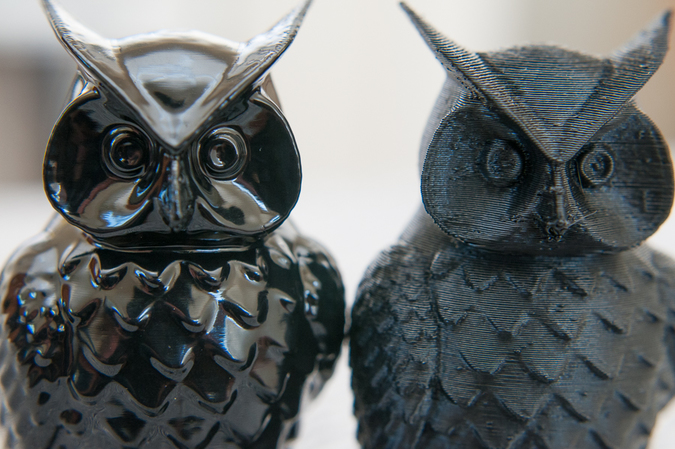
\includegraphics[width=\textwidth,cfbox=azul_marcos 4pt 0pt]{FOTOS/VAPORACETONA1}
    \end{subfigure}
    \qquad %add desired spacing between images, e. g. ~, \quad, \qquad, \hfill etc. 
      %(or a blank line to force the subfigure onto a new line)
    \begin{subfigure}[b]{0.4\textwidth}
        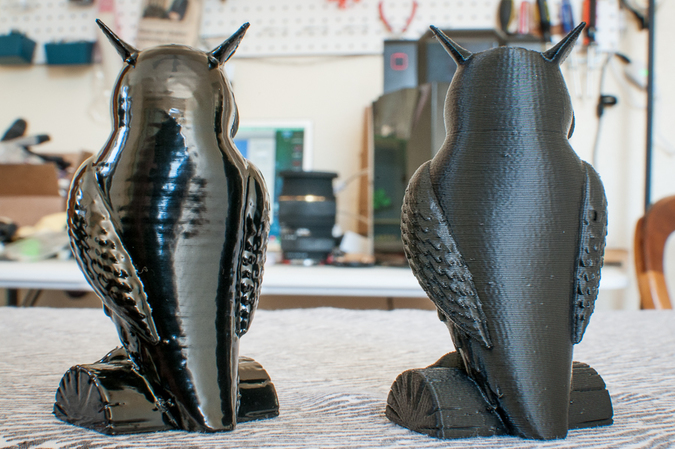
\includegraphics[width=\textwidth,cfbox=azul_marcos 4pt 0pt]{FOTOS/VAPORACETONA2}
    \end{subfigure}   
\end{figure}
Puede ser aplicada a mano, utilizando un pincel, pero también existe la posibilidad de crear una cámara casera de vapor de acetona relativamente sencilla.
\\\\
En los enlaces siguientes se describen 2 métodos diferentes de bañar con vapor de acetona piezas de ABS:
\\\\
\url{http://www.instructables.com/id/Safe-way-to-do-Acetone-bath/}\\\\
\url{http://sinkhacks.com/building-acetone-vapor-bath-smoothing-3d-printed-parts/}
\section{¿Quieres apoyar nuestro proyecto?}
Todos los miembros FFF World amamos la impresión 3D y la comunidad maker. Nos sentimos afortunados de poder trabajar en proyectos donde podamos entregar nuestra pasión sincera. En el futuro, nos gustaría poder desarrollar más materiales, más colores, más formatos. En definitiva, nos gustaría poder hacer crecer nuestra empresa.
\\\\
Para ello, una de las principales acciones para ayudarnos, si quieres hacerlo y estás satisfecho con el filamento, es la de votarnos en Amazon con 5 estrellas.
\begin{figure}[H]
\centering

\includegraphics[width=0.5\textwidth,cfbox=azul_marcos 1pt 0pt]{FOTOS/AMAZON_FIVE_STARS}
\caption*{¡Muchas gracias!}
\end{figure}
\subsection{Otros materiales con propiedades fantásticas disponibles en Amazon}
\begin{description}
\item[FlexiSMART Tech:] Diseñado para resistir a la abrasión y al desgaste de impresiones técnicas.
\item[ABS Tech:] Efecto warping minimizado. Alto rendimiento en aplicaciones técnicas.
\item[PETG Tech:] Máxima resistencia mécanica. Resistente al contacto con el agua y los rayos UV. Apto para uso alimentario.
\item[FilaMETAL:] PLA con carga metálica no abrasiva que da un acabado metálico espectacular a tus impresiones.
\item[PC Tech:] Policarbonato con gran resistencia a la temperatura y con excelentes propiedades mecánicas.
\item[Nylon Tech:] Imprimible a baja temperatura. Resistencia a los golpes con cierto grado de flexibilidad.
\item[PVA Tech:] Filamento soluble en agua indicado para uso como material de soporte. Excelente compatibilidad con PLA.
\item[HIPS Tech:] Filamento soluble en limoneno indicado para uso como material de soporte. Buena resistencia mecánica y excelente compatibilidad con ABS.
\end{description}
%\section{Bibliografía}
%Esta guía no habría sido posible sin el conocimiento libre generado por la comunidad RepRap. Para la elaboración de esta guía se han %utilizado imágenes y contenido extraidos de los siguientes sitios web.
%\\\\
%\url{http://www.gyrobot.co.uk/blog/how-to-3d-print-with-flexible-filaments}\\
%\url{http://www.thingiverse.com/thing:1496895}\\
%\url{http://www.thingiverse.com/thing:247024}\\
%\url{http://www.thingiverse.com/thing:16319}\\
%\url{http://www.thingiverse.com/thing:779011}\\
%\url{http://www.thingiverse.com/thing:1102900}\\
%\url{http://www.thingiverse.com/thing:147705}\\
%\url{http://www.thingiverse.com/thing:222667}\\
%\url{http://www.thingiverse.com/thing:512338}\\
%\url{https://all3dp.com/common-3d-printing-problems-and-their-solutions/}\\
%\url{https://www.simplify3d.com/support/}\\
%\url{http://www.thingiverse.com/thing:508896}\\
%\url{http://www.thingiverse.com/thing:1187344}

\includepdf{PDF/ES_CONTRAPORTADA.pdf}
\end{document}
